\documentclass[../main.tex]{subfiles}

\begin{document}

    En este capítulo definiremos un tercer acercamiento a las gramáticas de los lenguajes naturales desarrollado por Joachim Lambek en 1999 \cite{lambek99}. \\
    Un pregrupo es una estructura algebraica $(P,\leq,1, -^r,- ^l)$ que satisface las siguientes propiedades
        \begin{itemize}
            \item $(P, \geq)$ es un orden parcial;
            \item $(P,\cdot,1)$ es un monoide;
            \item Para cualesquiera $x,y,z \in P$, si $x \leq y$, entonces $x\cdot z \leq y \cdot z$; y
            \item para cualquier objeto $t \in P$,
            \begin{itemize}
                \item $t \cdot t^r \leq 1$ y $t^l \cdot t \leq 1$ (contracciones), y
                \item $1 \leq t^r \cdot t$ y $1 \leq t \cdot t^l$ (expansiones).
            \end{itemize}
        \end{itemize}
    Dado un conjunto de tipos gramáticales, por ejemplo, $B=\{ n,s \}$ podemos considerar el pregrupo libre generado por $B$ y dada la asignación de tipos ''Octavio'', ''envió'', ''una'' y ''carta'' dada por $n, n^r \cdot s \cdot n^l, n\cdot n^l$ y $n$ respectivamente, tenemos que
    \begin{align*}
        n \cdot (n^r \cdot s \cdot n^l) \cdot (n\cdot n^l) \cdot n &= (n \cdot n^r) \cdot s \cdot (n^l \cdot n)  \cdot (n^l \cdot n) \\
        &=1 \cdot s \cdot 1 \cdot 1 & \text{aplicando contracciones} \\
        &=s
    \end{align*}
    En estas gramáticas determinar si una oración es o no válida se puede decidir mediante operaciones algebraicas. Su uso es conveniente\footnote{Lambek además mencionaría que son prácticas, escribir operaciones algebraicas ocupan menos espacio y tiempo, que árboles de derivación o diagramas de automátas} ya que son tan expresivas como las gramáticas Lambek, no pierden compromiso con el principio de composicionalidad y determinar si una palabra pertenece a la gramática es no sólo decidible, sino que es requiere tiempo polinomial. \\
    Para la descripción de los pregrupos en el marco de la teoría de categorías, introduciremos el concepto de elementos adjuntos derechos e izquierdos en una categoría, que se traducen como \textit{cups} y $\textit{caps}$ en el lenguaje gráfico de categorías, para definir el concepto de una categoría rígida y las gramáticas que producen.  
    \section{Categorías rígidas}
        
	\begin{dfn}
		Una signatura rígida $G$ es una colección de generadores $G_1$ y tipos básicos $G_0$ junto a un par de funciones: \\
		$$\signature{G_1}{P(G_0)}$$
		donde $P(G_0)$ es el conjunto de tipos de pregrupos dados por la siguiente definición
		
		$$T(G_0) ::== a, b \in G_0 | a^r | a^l$$
		Un morfismo de signaturas rígidas $\varphi : G \to \Gamma$ es un par de funciones $\varphi_0 : G_0 \to \Gamma_0$ y $\varphi_1 : G_1 \to \Gamma_1$ tales que hacen conmutar el diagrama de signaturas. A la categoría de signaturas rígidas le llamamos \textbf{RgSig}.
	\end{dfn}
	\begin{dfn}
		Sea $(\mathcal{C}, \otimes, 1)$ una categoría monoidal. Un objeto $a^l$ es un adjunto izquierdo de un objeto $a$ y $a^r$ es adjunto derecho de $a$ si existen morfismos
		$$\eta_r: 1 \to a^r \otimes a \qquad \qquad \varepsilon_r : a \otimes a^r \to 1$$
		$$\eta_l: 1 \to a \otimes a^l \qquad \qquad \varepsilon_l : a^l \otimes a \to 1$$
		llamados las unidades y evaluaciones respectivamente, tales que hacen conmutar los siguientes triángulos 
            \begin{equation}
                \label{eq:snake}
    		\begin{tikzcd}
    			a \arrow{r}{\eta_l \otimes Id} \arrow[swap]{dr}{\id_a} & a \otimes a^l \otimes a \arrow{d}{\id \otimes \varepsilon_l}
    			& & 
    			a \arrow{r}{\id_a \otimes \eta_r} \arrow[swap]{dr}{\id_a} & a \otimes a^r \otimes a \arrow{d}{\varepsilon_r \otimes Id}\\
    			& a
    			& & &
    			a
    		\end{tikzcd}
            \end{equation}
	\end{dfn}
	\noindent Con base a la noción de adjuntos, podemos definir la clase de categorías que protagonizarán el presente capítulo. 
	\begin{dfn}
		Una categoría monoidal $(\mathcal{C}, \otimes, 1)$ es una categoría rígida si cada objeto $a$ tiene un adjunto izquierdo $a^l$ y un adjunto derecho $a^r$. 
	\end{dfn}
	\noindent Antes de continuar, desarrollemos un lenguaje gráfico para las categorías rígidas. En el capítulo $4$, establecimos como representar cada objeto y morfismo de una categoría monoidal por medio de diagramas, entonces basta ver cómo lo haremos con adjuntos, unidades y evaluaciones. \\
	El adjunto izquierdo lo representaremos mediante un cable con una flecha hacia arriba, mientras que el adjunto derecho también será una cable pero con una flecha hacia abajo, tal como mostramos a continuación.
    \begin{center}
        \begin{figure}[H]
		\includegraphics[scale=.2]{TeX/diagrama/5-1.pdf}
		\centering
	\end{figure}
    \end{center}
	Con esta convención, resulta natural dibujar los morfismos $\eta_l:1 \to a \otimes a^l$ y $\epsilon_l : a^l \otimes a \to 1$ de la siguiente manera
        \begin{center}
        \begin{figure}[H]
		\includegraphics[scale=.2]{TeX/diagrama/5-2.pdf}
		\centering
	   \end{figure}
        \end{center}
    \noindent Dada esta representación gráfica es común referirse a la unidad y evaluación con los nombres \textit{caps} y \textit{cups.} Por su parte, la unidad y evaluación derecha se representan de esta forma
    \begin{center}
        \begin{figure}[H]
		\includegraphics[scale=.2]{TeX/diagrama/5-3.pdf}
		\centering
	   \end{figure}
        \end{center}
    Con la cual las ecuaciones \eqref{eq:snake} adquieren la siguiente forma en el cálculo gráfico
    \begin{center}
        \begin{figure}[H]
		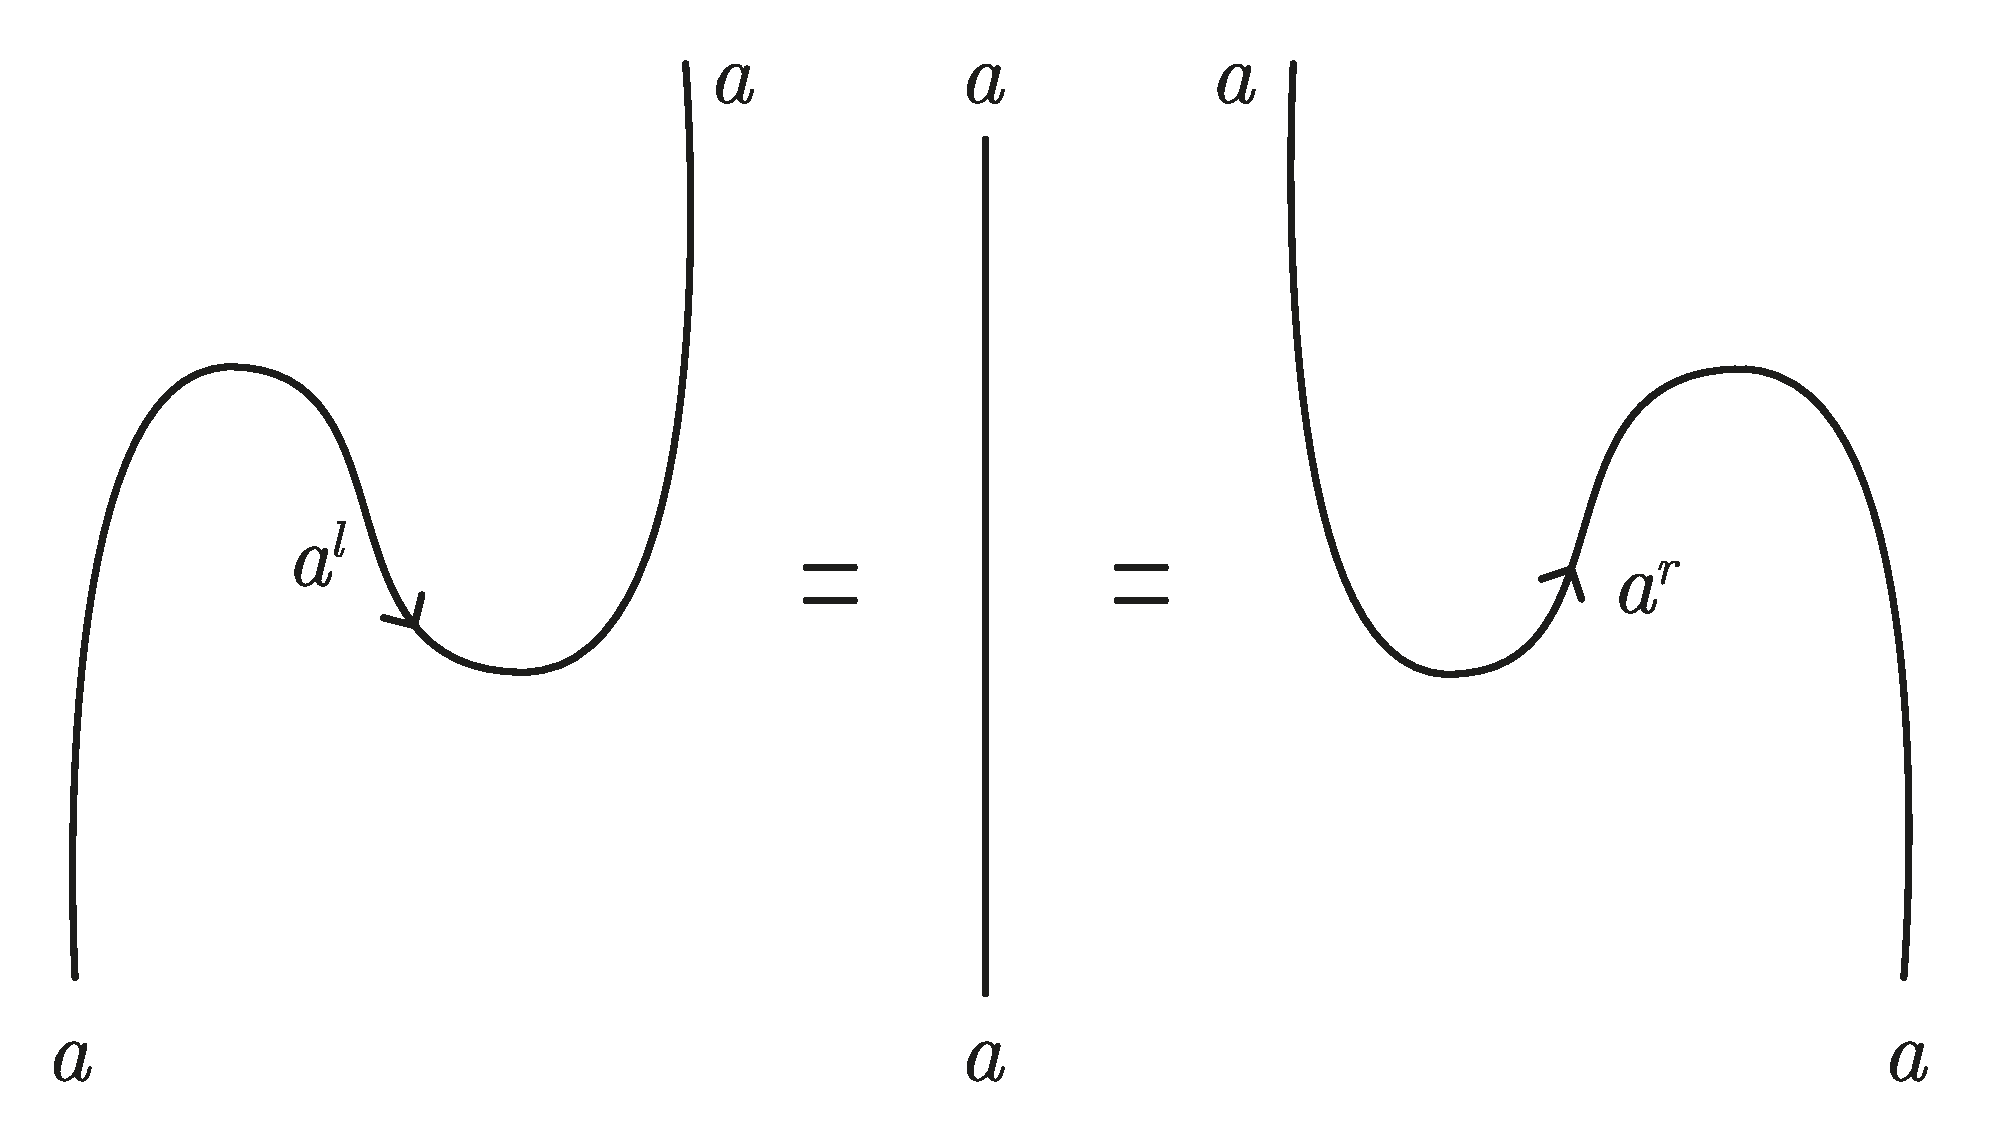
\includegraphics[scale=.2]{TeX/diagrama/5-4.pdf}
		\centering
	   \end{figure}
        \end{center}
    Debido a esta representación, estas ecuaciones son conocidas como las ecuaciones de la serpiente. \\

    Como en los capítulos anteriores, describiremos el poder expresivo de las gramáticas que pueden definirse sobre una categoría rígida. Un primer acercamiento a la respuesta es que tienen, a lo más, tanto capacidad como las gramáticas categoriales de acuerdo a la siguiente proposición.  

    \begin{prop}
        Sea $(\mathcal{C}, \otimes, 1)$ una categoría  rígida, entonces $\mathcal{C}$ es bicerrada.  
    \end{prop}
    \begin{proof}
        Sea $(\mathcal{C}, \otimes , 1)$ una categoría rígida. \\
        Para $a$ y $b$ objetos de $\mathcal{C}$ definimos $a \backslash b = a^r \otimes b$ y $b/a = b \otimes a^l$.\\
        Queremos mostrar que existen isomorfismos naturales $\mathcal{C}(a,c\otimes b^l) \cong \mathcal{C}(a\otimes b, c) \cong \mathcal{C}(b, a^r\otimes c)$. \\
        Probaremos solamente que $\mathcal{C}(a,c\otimes b^l) \cong \mathcal{C}(a\otimes b, c)$ pues son análogos. \\
        Sean $a$, $b$ y $c$ objetos en $\mathcal{C}$, y sea $f:a \otimes b \to c$ morfismo. Consideremos la siguiente composición
        $$a \xrightarrow[]{\cong} a \otimes 1 \xrightarrow[]{\id_a \otimes \eta_b} a \otimes b \otimes b^l \xrightarrow[]{f \otimes \id_{b^l}} c \otimes b^l$$
        y denotemosla $\Phi (f):a \to c \otimes b^l$, es decir, tenemos una morfismo $\Phi: \mathcal{C}(a \otimes b, c) \to \mathcal{C}(a, c \otimes b^l)$. \\
        Busquemos $\Psi: \mathcal{C}(a, c \otimes b^l) \to \mathcal{C}(a \otimes b, c)$ la inversa de $\Phi$. Sea $g: a \to c \otimes b^l$ y definimos $\Psi(g)$ como la composición
        $$a \otimes b \xrightarrow[]{g \otimes \id_b} c \otimes b^l \otimes b \xrightarrow[]{\id_c \otimes \varepsilon_b} c \otimes 1 \xrightarrow[]{\cong} c$$
        Notemos que por la ecuación de la serpiente es claro que son inversas. Falta ver que es natural tanto en $a$ como en $c$. \\
        Para la naturalidad en $a$, sea $h:a' \to a$ morfismo, queremos que el siguiente diagrama conmuta 
        \[
            \begin{tikzcd}
                \mathcal{C}(a' \otimes b, c) \arrow{r}{\Phi} \arrow{d}{h \otimes Id_b} & \mathcal{C}(a',c \otimes b^l) \arrow{d}{h}\\
                \mathcal{C}(a \otimes b, c) \arrow{r}{\Phi} & \mathcal{C}(a,c \otimes b^l)
            \end{tikzcd}
        \]
        Sea $f:a' \otimes b$, tenemos que ver que las siguiente composiciones son iguales
        $$a' \xrightarrow[]{h} \underbrace{a \xrightarrow[]{\cong} a \otimes 1 \xrightarrow[]{\id_a \otimes \eta_b} a \otimes b \otimes b^l \xrightarrow[]{f \otimes \id_{b^l}} c \otimes b^l}_{\Phi(f)} $$
        $$\underbrace{a' \xrightarrow[]{\cong} a' \otimes 1 \xrightarrow[]{\id_a \otimes \eta_b} a' \otimes b \otimes b^l \xrightarrow[]{h \otimes \id_{b \otimes b^l}} a \otimes b \otimes b^l \xrightarrow[]{f \otimes \id_{b^l}} c \otimes b^l}_{\Phi(f \circ (h \otimes \id_{b^l}))}$$
        Por la ecuacion \ref{intLaw2} tenemos la siguiente igualdad
        $$(\id_a \circ \eta_b) \circ (h \otimes \id_1) = (h \otimes Id_{b \otimes b^l}) \circ (\id_{a'} \otimes \eta_b)$$
        y aplicando $f \otimes b^l$ tenemos la igualdad deseada y, por lo tanto, el diagrama conmuta. \\
        Para la naturalidad en $b$ sea $k : c \to c'$, veamos que el siguiente diagrama conmuta
        \[
            \begin{tikzcd}
                \mathcal{C}(a \otimes b, c) \arrow{r}{\Phi} \arrow{d}{k} & \mathcal{C}(a,c \otimes b^l) \arrow{d}{k \otimes \id_{b^l}}\\
                \mathcal{C}(a \otimes b, c') \arrow{r}{\Phi} & \mathcal{C}(a,c' \otimes b^l)
            \end{tikzcd}
        \]
        Sea $g: a \otimes b \to c$, queremos ver que la composición $ (k \otimes \id_{b^l})\circ \Phi(g) = \Phi(k\circ g)$, lo cual es cierto pues
        \begin{align*}
            (k \otimes \id_{b^l}) \circ \Phi(g) &= (k \otimes \id_{b^l}) \circ ((g \id_{b^l}) \circ (Id_a \otimes \eta_b))  \\
            &= ((k \otimes \id_{b^l}) \circ (g \id_{b^l})) \circ (Id_a \otimes \eta_b) \\
            &= ((k \circ g) \otimes \id_{b^l}) \circ (Id_a \otimes \eta_b) \\
            &= \Phi(k \circ g)
        \end{align*}
        y, por lo tanto, el diagrama conmuta. \\
        Por lo tanto, tenemos el isomorfismo natural $\mathcal{C}(a,c\otimes b^l) \cong \mathcal{C}(a\otimes b, c)$ y, de manera análoga, $\mathcal{C}(b,a^r\otimes c) \cong \mathcal{C}(a\otimes b, c)$. \\
        Por lo tanto, $\mathcal{C}$ es una categoría bicerrada. 
    \end{proof}

    Dada $G$ una signatura rígida, definimos la categoría rígida libre como
    $$\textbf{RC}(G) = \textbf{MC}(G\cup \{ cups,caps \})/ \sim_{serpiente}$$
    donde $\sim_{serpiente}$ es la relación inducida por las ecuaciones de la serpiente \ref{eq:snake}. En otras palabras, $\textbf{RC}(G)$ es la categoría monoidal libre donde añadimos como generadores las unidades y evaluacones, e igualamos los morfismos de acuerdo a las ecuaciones de la serpiente para que se satisfaga la definición de categoría rígida. \\

    Antes de mostrar las gramáticas generadas en las categorías rígidas, hablaremos de una clase de morfismos que tendrán un rol importante en la siguiente sección. \\

    Sea $f: x \to y$ un morfismo en $\textbf{RC}(G)$, consideremos la siguiente composición

    $$y^r \xrightarrow[]{\cong} 1 \otimes y^r \xrightarrow[]{\eta_x \otimes \id_{y^r}} x^r \otimes x \otimes y^r \xrightarrow[]{\id_{x^r} \otimes f \otimes \id_{y^r}} x^r \otimes y \otimes y^r \xrightarrow[]{\id_{x^r} \otimes \varepsilon_y} x^r$$

    Definimos $f^r:y^r \to x^r$ como $f^r = (\id_{x^r} \otimes \varepsilon_y) \circ (\id_{x^r} \otimes f \otimes \id_{y^r}) \circ (\eta_x \otimes \id_{y^r})$ y gráficamente lo representamos como 
    \begin{center}
        \includegraphics[scale=.3]{TeX/diagrama/5-6.pdf}
    \end{center}

    Y, además, probemos que $f^r$ hace conmutar los siguientes diagramas
    \begin{multicols}{2}
        \begin{equation*}
            \begin{tikzcd}
                x\otimes y^r \arrow{r}{f \otimes \id_{y^r}} \arrow[swap]{d}{\id_x \otimes f^r} \arrow[dashed]{dr}{\varepsilon_f} & y \otimes y^r \arrow{d}{\varepsilon_y} \\
                x \otimes x^r \arrow[swap]{r}{\varepsilon_x} & 1
            \end{tikzcd}
        \end{equation*}
    
        \begin{equation*}
            \begin{tikzcd}
                1 \arrow{r}{\eta_x} \arrow[swap]{d}{\eta_y} \arrow[dashed]{rd}{\eta_f} & x^r \otimes x \arrow{d}{\id_{x^r} \otimes f} \\
                y^r \arrow[swap]{r}{f^r \otimes \id_y} \otimes y & x^r \otimes y
            \end{tikzcd}
        \end{equation*}
    \end{multicols}
    Primero veamos que el primer cuadrado conmuta
    \begin{align*}
        \varepsilon_x \circ (\id_x \otimes f^r) &= \varepsilon_x \circ (\id_x \otimes  ((\id_{x^r} \otimes \varepsilon_y) \circ (\id_{x^r} \otimes f \otimes \id_{y^r}) \circ (\eta_x \otimes \id_{y^r})))  \\
        &= \varepsilon_x \circ (\id_x \otimes  ((\id_{x^r} \otimes (\varepsilon_y \circ (f \otimes \id_{y^r})) \circ (\eta_x \otimes \id_{y^r})))  \\
        &= \varepsilon_x \circ (\id_x \otimes  \id_{x^r} \otimes (\varepsilon_y \circ (f \otimes \id_{y^r})) \circ (\id_x \otimes \eta_x \otimes \id_{y^r}) \\
        &= (\varepsilon_y \circ (f \otimes \id_{y^r})) \circ (\varepsilon_x \otimes \id_x \otimes \id_{y^r}) \circ (\id_x \otimes \eta_x \otimes \id_{y^r}) \\
        &= (\varepsilon_y \circ (f \otimes \id_{y^r})) \circ ((\varepsilon_x \otimes \id_x) \circ (\id_x \otimes \eta_x )) \otimes \id_{y^r} \\
        &= \varepsilon_y \circ (f \otimes \id_{y^r}) \circ (\id_x \otimes \id_{y^r}) \\
        &= \varepsilon_y \circ (f \otimes Id_{y^r})
    \end{align*}
    Por lo tanto, el diagrama conmuta. \\
    Probemos ahora que el segundo cuadrado conmuta 
    \begin{align*}
        (f^r \otimes \id_y)\circ \eta_y &= (((\id_{x^r} \otimes \varepsilon_y) \circ (\id_{x^r} \otimes f \otimes \id_{y^r}) \circ (\eta_x \otimes \id_{y^r})) \otimes \id_y) \circ \eta_y \\
        &= (((\id_{x^r} \otimes \varepsilon_y) \circ ((\id_{x^r} \otimes f ) \circ \eta_x)\otimes \id_{y^r}) \otimes \id_y) \circ \eta_y \\
        &= (\id_{x^r} \otimes \varepsilon_y \otimes \id_y) \circ (((\id_{x^r} \otimes f) \circ \eta_x) \otimes \id_y \otimes \id_{y^r}) \circ \eta_y \\
        &= (\id_{x^r} \otimes \varepsilon_y \otimes \id_y) \circ (\id_{x^r} \otimes \id_y \otimes \eta_y) \circ ((\id_{x^r} \otimes f)\circ \eta_x) \\
        &= (\id_{x^r} \otimes ((\varepsilon_y \otimes \id_y)\circ(\id_y \otimes \eta_y))) \circ ((\id_{x^r} \otimes f)\circ \eta_x) \\
        &= (\id_{x^r} \otimes \id_y) \circ ((\id_{x^r} \otimes f)\circ \eta_x) \\
        &= (\id_{x^r} \otimes f)\circ \eta_x
    \end{align*}
    Por lo tanto el diagrama conmuta e introducimos la siguiente definición

    \begin{dfn}
        Sea $f:x \to y$ un morfismo en $\textbf{MC}(G)$, definimos la \textbf{contracción y expansión generalizada derecha de} $f$ como $\varepsilon_f : x \otimes y^r \to 1$ y $\eta_f : 1 \to x^r \otimes y$ dadas por 
        $$\varepsilon_f =\varepsilon_y \circ (f \otimes Id_{y^r}))= \varepsilon_x \circ (\id_x \otimes f^r) \qquad \qquad \text{ y } \qquad \qquad \eta_f=(\id_{x^r} \otimes f)\circ \eta_x = (f^r \otimes \id_y)\circ \eta_y$$ 
        Análogamente definimos la \textbf{contracción y expansión generalizada derecha de} $f$como $\varepsilon_f : y^l \otimes x \to 1$ y $\eta_f : 1 \to y \otimes x^l$ dadas por 
        $$\varepsilon_f = \varepsilon_y \circ (\id_{y^l}\otimes f) \qquad \qquad \qquad \qquad \text{\hspace{.7cm}y} \qquad \qquad \qquad \qquad \eta_f =(f \otimes \id_{x^l}) \circ \eta_x$$
        Los representamos gráficamente de la siguiente manera
        \begin{center}
        \includegraphics[scale=.2]{TeX/diagrama/5-7.pdf}
        \end{center}
        Finalmente llamaremos \textbf{paso inducido} a un morfismo de la forma $\id_u \otimes s \otimes \id_v : u \otimes x \otimes v \to u \otimes y \otimes v$ donde $s: x \to y$ es un morfismo generador. 
    \end{dfn}
    

    
    
    \section{Pregrupos}

    Definamos la noción de gramáticas sobre una categoría rígida, una subclase de las gramáticas bicerradas. 
    \begin{dfn}
        Una \textbf{gramática rígida} $G$ es una signatura rígida de la siguiente forma
        $$\signature{P(B+V)}{P(B+V)}$$
        donde $V$ es un vocabulario y $B$ un conjunto de tipos básicos. El lenguaje generado por $G$ se define como
        $\mathcal{L}(G) = \{ u \in V^* | \exists g :u \to s \in \textbf{RC}(G) \}$
        donde $\textbf{RC}(G)$ es la categoría rígida generada por $G$.
    \end{dfn}
    Con base a la definición anterior, podemos establecer una gramática de pregrupo, una gramática rígida donde cada palabra en el vocabulario tiene asignados tipos. 
    \begin{dfn}
        Una \textbf{gramática de pregrupo} es una tupla $G=(V,B, \Delta, I,s)$ donde $V$ es un vocabulario, $B$ es un conjunto finito de tipos básicos, $\Delta \subset V \times P(B)$ es un léxico que asigna a cada palabra un posible tipo de pregrupo, y $I \subset B \times B$  un conjunto finito de reglas de producción. El lenguaje generado por $G$ está dado por
        $\mathcal{L}(G) = \{ u \in V^* | \exists g :u \to s \in \textbf{RC}(G) \}$
        donde $\textbf{RC}(G) = \textbf{RC}(\Delta+I)$
    \end{dfn}
    \begin{ej}
        Sea $B = \{ s, n \} $ el conjunto de tipos básicos correspondiente oración y sustantivo con el siguiente léxico 
        $$\Delta(Octavio)=n \qquad \Delta(envi\acute{o}) =n^l \otimes n \otimes n \qquad \Delta(una)=n \otimes n^r \qquad \Delta(carta)=n$$
        $$\Delta (a)=s^l \otimes s \otimes n^r \qquad \Delta(su)=n^r \otimes n \qquad \Delta(amada)=n$$
        Entonces la oración ''Octavio envió una carta a su amada'' es gramaticalmente correcta dado el siguiente morfismo.
        \begin{figure}[H]		
            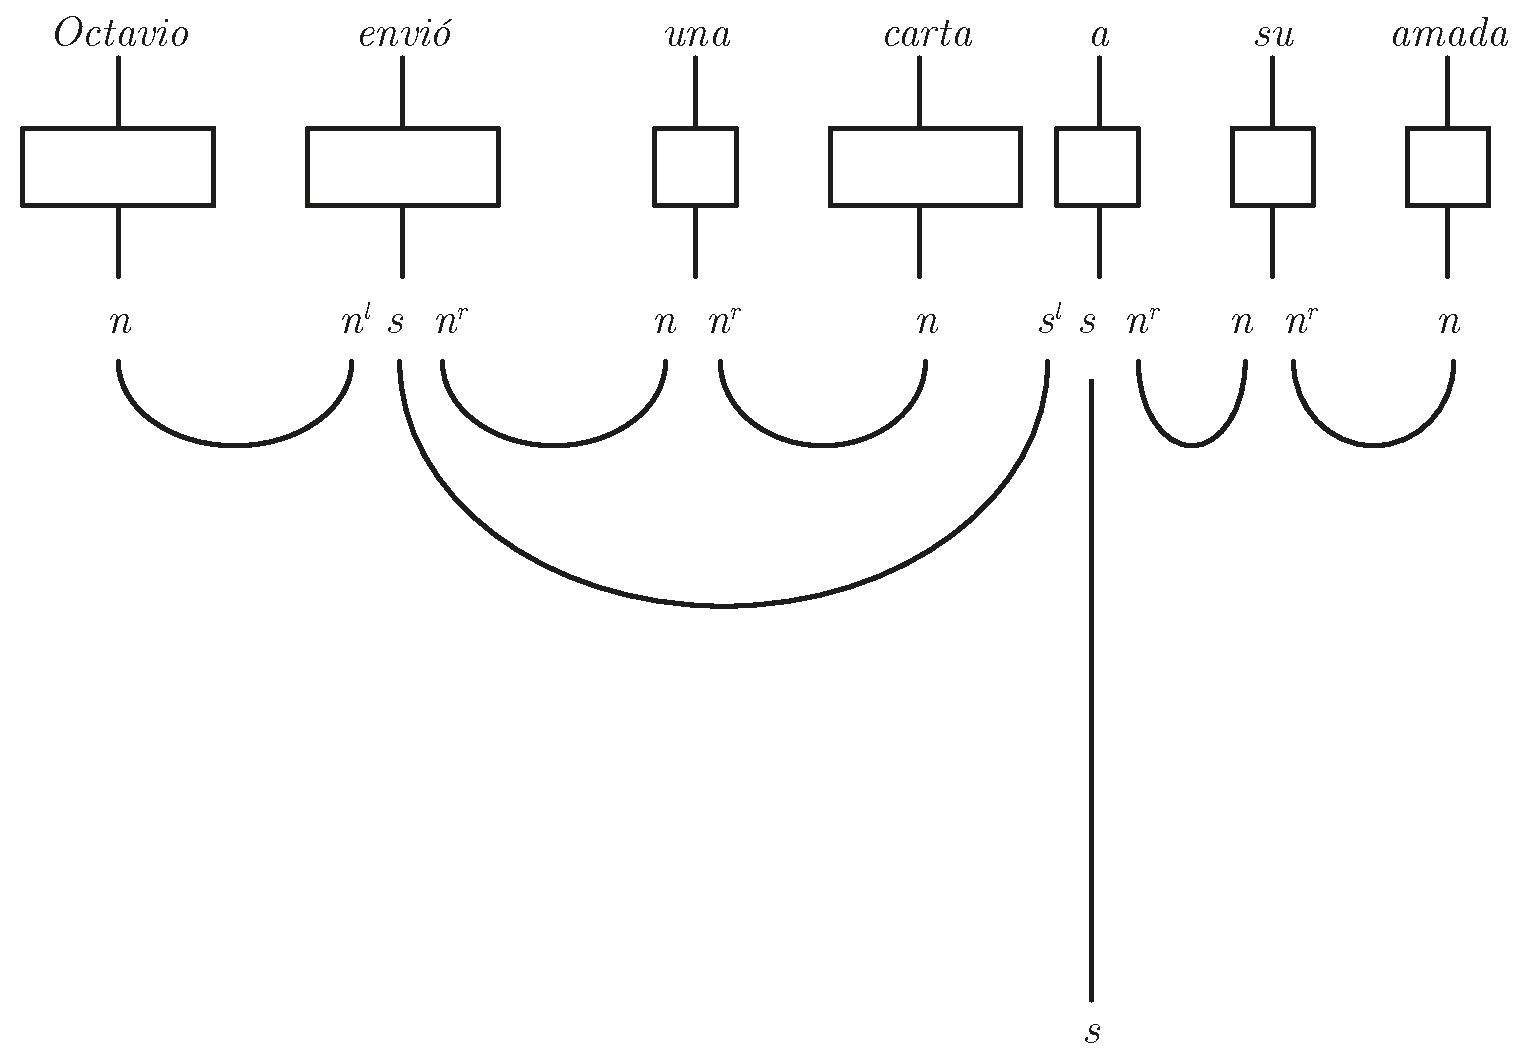
\includegraphics[scale=.45]{TeX/diagrama/pregroup.pdf}
			\centering
	\end{figure}        
    \end{ej}
    Anteriormente mencionamos que las gramáticas de pregrupos son, a lo más, tan expresivas como las gramáticas bicerradas. Pero el ejemplo anterior basado en \ref{gramAB} sugiere que poseen exactamente el mismo poder expresivo y. más aún, existe una reducción funtorial canónica como lo veremos a continuación. 
    \begin{prop}
        Sea $G$ una gramática de Lambek, entonces existe una gramática de pregrupo $G'$ con una reducción funtorial $\textbf{MC}(G) \to \textbf{RC}(G)$
    \end{prop}
    \begin{proof}
        Sea $G$ una gramática de Lambek. Consideremos $G'$ la gramática de pregrupos con el vocabulario, tipos básicos y léxico que $G'$ con las reglas de producción dadas por la siguiente traducción entre gramáticas
        \begin{center}
            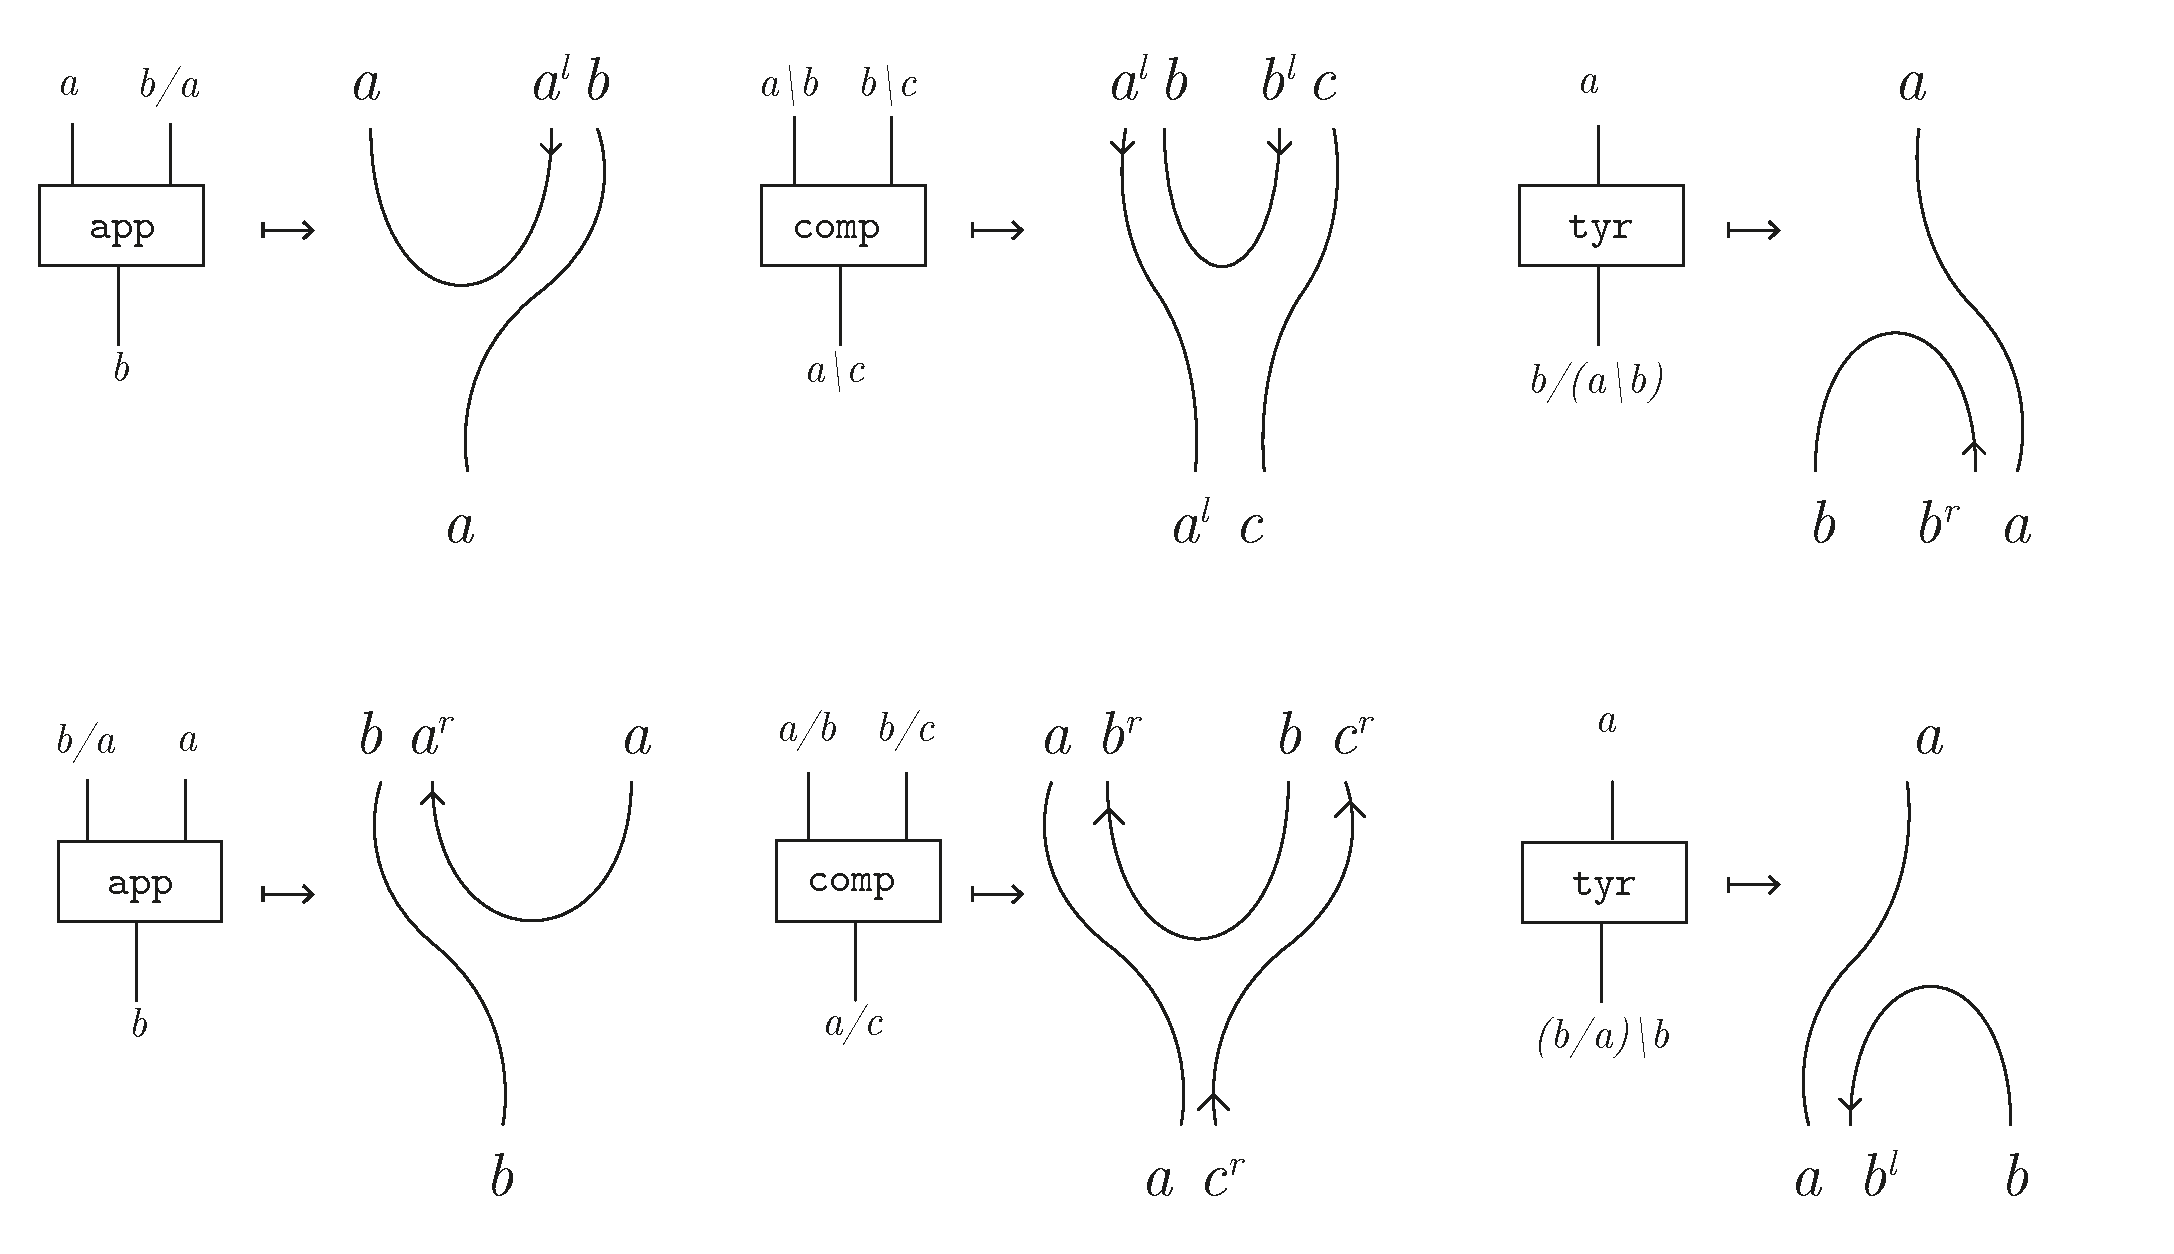
\includegraphics[scale=.38]{TeX/diagrama/5-5.pdf}
        \end{center}
    \end{proof}

    El estudio de gramáticas de pregrupos es entonces el estudio de las gramáticas descritas en el capítulo anterior, sin embargo, la validación computacional de oraciones aceptadas por el lenguaje es computacionalmente más eficiente de acuerdo al \textit{Switching lemma} probado por Lambek y Teller en \cite{lambek99}. Antes de enunciarlo, veamos los siguientes movimientos válidos en una categoría rígida.

    \begin{enumerate}
            \item Los generadores de $f:x \to y$ y $g:a \to b$ no comparten elementos en el codominio y dominio respectivamente, entonces podemos intercambiar el orden de composición de $f$ y $g$ según convenga, de acuerdo a la ley de intercambio. 
            \item Reemplazar dos pasos inducidos por un solo paso inducido. \\
            Supongamos $d_1 = \id_u \otimes g \otimes \id_v$ y $d_2 = \id_u \otimes h \otimes \id_v$ con $f:x \to y$ y $h:y \to z$, entonces $d_2 \circ d_1 = (\id_u \otimes h \otimes \id_v) \circ (\id_u \otimes g \otimes \id_v) = \id_u \otimes (h \circ g) \otimes \id_v$.
            \item Reemplazar una expansión generalizada seguida por una contracción generalizada por un paso inducido. Tenemos dos casos:
            \begin{enumerate}
                \item La contracción generalizada está a la derecha. Gráficamente tenemos el siguiente caso 
                \begin{center} \includegraphics[scale=.2]{TeX/diagrama/5-8.pdf}
                \end{center}
                Sea $f:y \to x$ y $g:z \to y$, entonces tenemos que 
                \begin{align*}
                    (\id_{z^r}\otimes \varepsilon_f) \circ (\eta_g \otimes \id_{x^r}) &= (\id_{z^r} \otimes (\varepsilon_x \circ (f \otimes \id_{x^r}))) \circ (((\id_{z^r} \otimes g) \circ \eta_z)\otimes \id_{x^r} ) \\
                    &= (\id_{z^r} \otimes \varepsilon_x) \circ (\id_{z^r} \otimes f \otimes \id_{x^r}) \circ (\id_{z^r} \otimes g \otimes \id_{x^r}) \circ (\eta_{z^r} \otimes \id_{x^r}) \\
                    &= (\id_{z^r} \otimes \varepsilon_x) \circ (\id_{z^r} \otimes (f\circ g) \otimes \id_{x^r}) \circ (\eta_{z^r} \otimes \id_{x^r}) \\
                    &= (f \circ g)^r
                \end{align*}
                Por lo tanto, $\id_u \otimes (\id_{z^r}\otimes \varepsilon_f) \circ (\eta_g \otimes \id_{x^r}) \otimes \id_v = \id_u \otimes (f \circ g)^r \otimes \id_v $. \\
                \item La contracción generalizada está a la izquierda. Gráficamente tenemos el siguiente caso
                \begin{center} \includegraphics[scale=.2]{TeX/diagrama/5-9.pdf}
                \end{center}
                Sea $f:y \to x$ y $g:x \to y$, entonces

                \begin{align*}
                    (\varepsilon_g \circ \id_z) \circ (\id_x \circ \eta_f) &= ((\varepsilon_y \circ (g \otimes \id_{y^r}))\otimes \id_{z}) \circ (\id_x \otimes ((\id_{y^r} \otimes f) \circ \eta_y)) \\
                    &= (\varepsilon_y \otimes \id_z) \circ (g \otimes \id_{y^r} \otimes \id_z) \circ (\id_x \otimes \id_{y^r} \otimes f) \circ (\id_x \otimes \eta_y) \\
                    &= (\varepsilon_y \otimes \id_z) \circ (\id_y \otimes \id_{y^r} \otimes f) \circ (g \otimes \id_{y^r} \otimes \id_y) \circ (\id_x \otimes \eta_y) \\
                    &= f \circ (\varepsilon_y \otimes \id_y) \circ (\id_y \otimes \eta_y) \circ g \\
                    &= f \circ \id_y \circ g \\
                    &= f \circ g
                \end{align*}
                Por lo tanto, $\id_u \otimes ((\varepsilon_g \circ \id_z) \circ (\id_x \circ \eta_f)) \otimes \id_v = \id_u \otimes f \circ g \otimes \id_v$
            \end{enumerate}
        Notemos que estos dos casos corresponden a generalizaciones de las ecuaciones de la serpiente.  
        \item Reemplazar un paso inducido seguido por una contracción generalizada por una contracción generalizada. Tenemos dos subcasos:
        \begin{enumerate}
            \item El paso inducido está a la izquierda. 
            \begin{center} \includegraphics[scale=.2]{TeX/diagrama/5-10.pdf}
                \end{center}
            Sea $f: y \to x$ y $g:z \to y$. Entonces
            \begin{align*}
                \varepsilon_{f \circ g} &= \varepsilon_x \circ ((f\circ g) \otimes \id_{x^r})  \\
                &= \varepsilon_x \circ ((f \otimes \id_{x^r}) \otimes (g \otimes \id_{x^r})) \\
                &= (\varepsilon_x \circ (f \otimes \id_{x^r})) \circ (g \otimes \id_{x^r}) \\
                &= \varepsilon_f \circ (g \otimes \id_{x^r})
            \end{align*}
            Por lo tanto, $\id_u \otimes \varepsilon_{f \circ g} \otimes \id_v = \id_u \otimes (\varepsilon_f \circ (g \otimes Id_x)) \otimes \id_v$
            \item El paso inducido está a la derecha. 
            \begin{center} \includegraphics[scale=.2]{TeX/diagrama/5-11.pdf}
            \end{center}
            Sea $f:z \to x$ y $g: y \to z$. 
            \begin{align*}
                \varepsilon_{f \circ g} &= \varepsilon_x \circ ((f \circ g) \otimes \id_{x^r}) \\
                &= \varepsilon_x \circ ((f \circ \id_y \circ g) \otimes \id_{x^r}) \\
                &= \varepsilon_x \circ (f \otimes \id_x) \circ (\id_y \otimes \id_{x^r}) \circ (g \otimes \id_{x^r}) \\
                &= \varepsilon_x \circ (f \otimes \id_{x^r}) \circ [((\varepsilon_z \otimes \id_z) \circ (\id_z \otimes \eta_z) ) \otimes \id_{x^r}] \circ (g \otimes \id_{x^r}) \\
                &= \varepsilon_x \circ (f \otimes \id_{x^r}) \circ (\varepsilon_z \otimes \id_z \otimes \id_{x^r}) \circ (\id_z \otimes \eta_z \otimes \id_{x^r}) \circ (g \otimes \id_{x^r}) \\
                &= \varepsilon_x \circ (\id_x \otimes \id_{x^r}) \circ (\varepsilon_z \otimes f \otimes \id_{x^r}) \circ (g \otimes \eta_z \otimes \id_{x^r}) \circ (\id_y \otimes \id_{x^r}) \\
                &=\varepsilon_x \circ (\varepsilon_z \otimes f \otimes \id_{x^r}) \circ (g \otimes \eta_z \otimes \id_{x^r}) \\
                &=\varepsilon_x \circ (\varepsilon_z \otimes \id_x \otimes \id_{z^r}) \circ (\id_z \otimes \id_{z^r} \otimes f \otimes \id_{x^r}) \circ (g \otimes \eta_z \otimes \id_{x^r}) \\
                &=\varepsilon_z \circ (\id_z \otimes \id_{z^r} \otimes \varepsilon_x) \circ (\id_z \otimes \id_{z^r} \otimes f \otimes \id_{x^r}) \circ (g \otimes \eta_z \otimes \id_{x^r}) \\
                &=\varepsilon_z \circ (\id_z \otimes \id_{z^r} \otimes \varepsilon_x) \circ (g \otimes \id_{z^r} \otimes f \otimes \id_{x^r}) \circ (\id_y \otimes \eta_z \otimes \id_{x^r}) \\
                &=\varepsilon_z \circ (g \otimes \id_{z^r} \otimes \varepsilon_x) \circ (\id_y \otimes \id_{z^r} \otimes f \otimes \id_{x^r}) \circ (\id_y \otimes \eta_z \otimes \id_{x^r}) \\
                &=\varepsilon_z \circ (g \otimes \id_{z^r}) \circ (\id_y \otimes \id_{z^r} \otimes \varepsilon_x) \circ (\id_y \otimes \id_{z^r} \otimes f \otimes \id_{x^r}) \circ (\id_y \otimes \eta_z \otimes \id_{x^r}) \\
                &= \varepsilon_g \circ [\id_y \otimes ((\id_{z^r} \otimes \varepsilon_x) \circ (\id_{z^r} \otimes f \otimes \id_{x^r}) \circ (\eta_z \otimes \id_{x^r}))] \\
                &= \varepsilon_g \circ (\id_y \otimes f^r)
            \end{align*}
        Y, por lo tanto, $\id_u \otimes \varepsilon_{f \circ g} \otimes \id_v = \varepsilon_g \circ (\id_y \otimes f^r)$
        \end{enumerate}
        \item Reemplazar una expansión generalizada seguida por un paso inducido por una expansión generalizada. Tenenemos nuevamente dos susbcasos:
        \begin{enumerate}
            \item El paso inducido está a la derecha
            \begin{center} \includegraphics[scale=.2]{TeX/diagrama/5-12.pdf}
            \end{center}
            \item El paso inducido está a la izquierda
            \begin{center} \includegraphics[scale=.2]{TeX/diagrama/5-13.pdf}
            \end{center}
        \end{enumerate}
        \end{enumerate}

    \begin{thm}
        Sea $G$ una gramática de pregrupo y $f$ un morfismo en $\textbf{RC}(G)$, entonces $f$ puede expresar como
        $$f= (e_1 \circ \cdots \circ e_r) \circ (p_1 \circ \cdots \circ p_s) \circ (c_1 \circ \cdots \circ c_t)$$
        donde los $e_i$ son expansiones generalizadas, los $p_j$ son pasos inducidos y $c_k$ son contracciones generalizadas.
    \end{thm}


    \begin{proof}
        Sea $G$ una gramática de pregrupo y $f: u \to v$ un morfismo en $\textbf{RC}(G)=\textbf{RC}(\Delta_G+I_G)$, entonces de acuerdo a la proposición \ref{freemonoidal}, $f$ se expresa como un diagrama en posición general, $f=d_n \circ d_{n-1} \circ \cdots \circ d_2 \circ d_1$, hagamos la prueba por inducción sobre $n$. \\
        Si $n=1$ terminamos. Supongamos que si tenemos un diagrama con $n$ niveles, entonces satisface el teorema y supongamos $f= d_{n+1} \circ \cdots \circ d_1$. \\
        Aplicamos la hipótesis de inducción al morfismo $d_n \circ \cdots \circ d_1$, entonces 
        $$d_n \circ \dots d_n =  c_1 \otimes \cdots \otimes c_r \otimes p_1 \otimes \cdots \otimes p_s \otimes e_1 \otimes \cdots \otimes e_t$$
        donde los $e_i$ son expansiones generalizadas, los $p_j$ son pasos inducidos y $c_k$ son contracciones generalizadas. \\
        Notemos que si $d_n$ es una expansión generalizada, entonces ya terminamos. Supongamos que no y tenemos los siguientes casos. 
        \begin{itemize}
            \item Caso 1. El dominio de $d_n$ no es codominio de expansiones, contracciones generalizadas o pasos inducidos. Entonces, podemos aplicar consecutivamente el movimiento $1.$ para llevarlo a la forma deseada. 
            \item Caso 2. El dominio de $d_n$ es codominio de una expansión generalizada $c_i$. Entonces podemos aplicar el movimiento $1.$ para poner consecutivamente $d_n \circ c_i$.
            \begin{itemize}
                \item Caso 2.1. $d_n$ es paso inducido. Entonces podemos aplicar el movimiento $5.a)$ o $5.b)$ para poner una expansión generalizada. 
                \item Caso 2.2. $d_n$ es una contracción generalizada. Entonce podemos aplicar $3.a)$ 0 $3.b)$ para sustutuir $d_n \circ c_i$ por un paso inducido y, de ser necesario, aplicar el caso 1 o el caso 2.1
            \end{itemize}
            \item Caso 3. El dominio de $d_n$ es codominio de un paso inducido $p_j$. Entonces podemos aplicar consecutivamente el movimiento $1$ hasta obtener $d_n \circ p_j$ 
            \begin{itemize}
                \item Caso 3.1. $d_n$ es paso inducido, entonces ya terminamos. 
                \item Caso 3.2 $d_n$ es contracción generalizada, entonces podemos aplicar el movimiento $4.a)$ o $4.b)$ para obtener una contracción generalizada, y aplicar este paso consecutivamente hasta poder aplicar el movimiento $1$ y mover la contracción según la configuración deseada.
            \end{itemize}
        \end{itemize}
        Notemos finalmente que el dominio $d_n$ no puede ser el codominio de una contracción generalizada, pues sería la identidad en $1$ o una expansión generalizada. \\
        Por lo tanto, en cualquier caso $f$ es expresable de la forma deseada como queríamos demostrar. 
    \end{proof}
    Un corolario inmediato de este lema es el siguiente
    \begin{cor}
        Sea $G=(V,B, \Delta,I,s)$ una gramática de pregrupo y $u \in \mathcal{L}(G)$, entonces existe una derivación de $f:u \to s$ usando exclusivamente pasos inducidos y contracciones generalizadas.
        
    \end{cor}
    \begin{proof}
        Sea $G=(V,B, \Delta,I,s)$ una gramática de pregrupo y $u \in \mathcal{L}(G)$, entonces existe un morfismo $f:u \to s$, por el teorema anterior, 
         $$f= (e_1 \circ \cdots \circ e_r) \circ (p_1 \circ \cdots \circ p_s) \circ (c_1 \circ \cdots \circ c_t): u \to s$$
        donde los $e_i$ son expansiones generalizadas, los $p_j$ son pasos inducidos y $c_k$ son contracciones generalizadas. \\
        Supongamos que $r>0$, entonces ya que $\cod(e_1)=v\otimes a \otimes b^r \otimes w$ con $a,b \in V \cup B$ y $v,w \in (V \cup B)^*$, ya que $e_2$, ..., $e_r$ son contracciones, entonces $\cod(f)=v' \otimes a \otimes b^r \otimes w'$, entonces $\cod (f) \neq s$, pues $s \in V \cup B$. \\
        Por lo tanto, $r=0$ y $f=(p_1 \circ \cdots \circ p_s) \circ (c_1 \circ \cdots \circ c_t)$.
    \end{proof}
    El colorario anterior nos brinda la ventaja principal de los pregrupos sobre las gramáticas anteriores; el análisis de la sintaxis mediante estas gramáticas es más eficiente, pues existe un pseudoalgoritmo para realizar las reducciones. Más aún, es ejecutable en tiempo polinomial \cite{Degeilh2005} 
\end{document}